\PassOptionsToPackage{unicode=true}{hyperref} % options for packages loaded elsewhere
\PassOptionsToPackage{hyphens}{url}
%
\documentclass[
]{book}
\usepackage{lmodern}
\usepackage{amssymb,amsmath}
\usepackage{ifxetex,ifluatex}
\ifnum 0\ifxetex 1\fi\ifluatex 1\fi=0 % if pdftex
  \usepackage[T1]{fontenc}
  \usepackage[utf8]{inputenc}
  \usepackage{textcomp} % provides euro and other symbols
\else % if luatex or xelatex
  \usepackage{unicode-math}
  \defaultfontfeatures{Scale=MatchLowercase}
  \defaultfontfeatures[\rmfamily]{Ligatures=TeX,Scale=1}
\fi
% use upquote if available, for straight quotes in verbatim environments
\IfFileExists{upquote.sty}{\usepackage{upquote}}{}
\IfFileExists{microtype.sty}{% use microtype if available
  \usepackage[]{microtype}
  \UseMicrotypeSet[protrusion]{basicmath} % disable protrusion for tt fonts
}{}
\makeatletter
\@ifundefined{KOMAClassName}{% if non-KOMA class
  \IfFileExists{parskip.sty}{%
    \usepackage{parskip}
  }{% else
    \setlength{\parindent}{0pt}
    \setlength{\parskip}{6pt plus 2pt minus 1pt}}
}{% if KOMA class
  \KOMAoptions{parskip=half}}
\makeatother
\usepackage{xcolor}
\IfFileExists{xurl.sty}{\usepackage{xurl}}{} % add URL line breaks if available
\IfFileExists{bookmark.sty}{\usepackage{bookmark}}{\usepackage{hyperref}}
\hypersetup{
  pdftitle={A Person-Centered Framework},
  pdfauthor={Various authors},
  pdfborder={0 0 0},
  breaklinks=true}
\urlstyle{same}  % don't use monospace font for urls
\usepackage{longtable,booktabs}
% Allow footnotes in longtable head/foot
\IfFileExists{footnotehyper.sty}{\usepackage{footnotehyper}}{\usepackage{footnote}}
\makesavenoteenv{longtable}
\usepackage{graphicx,grffile}
\makeatletter
\def\maxwidth{\ifdim\Gin@nat@width>\linewidth\linewidth\else\Gin@nat@width\fi}
\def\maxheight{\ifdim\Gin@nat@height>\textheight\textheight\else\Gin@nat@height\fi}
\makeatother
% Scale images if necessary, so that they will not overflow the page
% margins by default, and it is still possible to overwrite the defaults
% using explicit options in \includegraphics[width, height, ...]{}
\setkeys{Gin}{width=\maxwidth,height=\maxheight,keepaspectratio}
\setlength{\emergencystretch}{3em}  % prevent overfull lines
\providecommand{\tightlist}{%
  \setlength{\itemsep}{0pt}\setlength{\parskip}{0pt}}
\setcounter{secnumdepth}{5}
% Redefines (sub)paragraphs to behave more like sections
\ifx\paragraph\undefined\else
  \let\oldparagraph\paragraph
  \renewcommand{\paragraph}[1]{\oldparagraph{#1}\mbox{}}
\fi
\ifx\subparagraph\undefined\else
  \let\oldsubparagraph\subparagraph
  \renewcommand{\subparagraph}[1]{\oldsubparagraph{#1}\mbox{}}
\fi

% set default figure placement to htbp
\makeatletter
\def\fps@figure{htbp}
\makeatother

\usepackage{booktabs}
\usepackage[]{natbib}
\bibliographystyle{apalike}

\title{A Person-Centered Framework}
\author{Various authors}
\date{2020-03-26}

\begin{document}
\maketitle

{
\setcounter{tocdepth}{1}
\tableofcontents
}
\hypertarget{reason}{%
\chapter{Reason}\label{reason}}

This framework comes from a simple starting point: the intent of supports and services is to help each person to flourish, to achieve a better life.

That belief is, thankfully, not a new one. It aligns with the MDHHS person-centered planning policy\citep{pcp-policy}, which begins by stating that:

\begin{quote}
\emph{The purpose of the community mental health system is to support adults and children\ldots{} to live successfully in their communities --- achieving community inclusion and participation, independence, and productivity {[}and to{]} to identify and achieve their personal goals.}
\end{quote}

The framework defined below is an attempt to apply these longstanding and fundamental values in a way that allows for consistent definitions, implementation, and evaluation.

\hypertarget{goal}{%
\section{Goal}\label{goal}}

Each person's ability to choose a better future and map their journey toward it: this is what person-centered planning enables. In order for services to effectively support a person in this process, they must be provided within the context of a person's goals. Orienting a broad and complex system to keep the person at the center requires a consistent, overarching framework. MDHHS BHDDA is working to support this person-centered orientation with the following strategy:

\textbf{Goal:} To develop \protect\hyperlink{bok}{a common body of knowledge} for person-centered planning,
mapped to \protect\hyperlink{policy}{relevant policies} and \protect\hyperlink{research}{research},
which will inform a \protect\hyperlink{curriculum}{shared curriculum}
and \protect\hyperlink{measure}{measurement framework}
to support \protect\hyperlink{pcpdca}{improved quality of life} for each person.

\hypertarget{pcpdca}{%
\chapter{Person-Centered Planning (Doing, Checking, Acting)}\label{pcpdca}}

The collective effect of our needs and environments has a profound impact on society, but the primary catalyst for transformation is at the level of the individual person. This is the profound insight of \emph{person-centered planning} (PCP), which has long been the cornerstone of Michigan policy related to behavioral health services and supports.\footnote{See \citet{mi-mhc}.}

Despite the central position of PCP to the Medicaid services system in Michigan, in practice it has often been relegated to the planning meeting itself and the preparation for that meeting: ensuring inclusion of family and friends, personal involvement, etc. While the act of developing a plan remains a cornerstone of the process, it is only the first step of what is needed to truly achieve one's goals.\footnote{Part of the focus on the meeting is due to the auditing focus on the plan document: an instance of \emph{what is measured, is addressed}.}

In this document and in the work under development with MDHHS-BHDDA, the phrase \emph{person-centered planning} is used broadly, to encompass not only the initial planning process but also its implementation, monitoring, and refinement. The need for this definition to extend beyond the PCP meetings and to direct all services and supports is already recognized within state policy, which indicates that:\footnote{MDHHS BHDDA Person-Centered Planning Policy (June 5, 2017), p.~1}

\begin{quote}
\emph{through PCP, a person is engaged in decision-making, problem solving, monitoring progress, and making needed adjustments to goals and supports and services provided in a timely manner.}
\end{quote}

Since the intent of supports and services is to improve personal quality of life, practitioners can view the PCP process as similar to the \emph{Plan-Do-Check-Act} (PDCA) cycle, which involves each element of the broad scope of PCP defined above. Versions of the PDCA cycle have already been successfully incorporated into the supports and treatment planning process for people with varying conditions and needs, from intellectual and developmental disabilities, to mental illness, to physical health concerns.

If we want to understand whether an individual person's plan is supporting their goals, it is necessary to have a strategy to measure improvement in the person's desired areas of focus. Such measurement-based approaches have been gaining traction in their use across populations.\footnote{\citet{shalock-changes} notes ``an increased emphasis on\ldots{} conducting outcome evaluation\ldots{} to assess the degree to which personal goals, positive changes, or benefits have been achieved'' in IDD planning.}

Framing the intent of supports and services as improving personal quality of life through person-centered planning also creates a natural bridge to using well-tested quality improvement processes at the individual level. Perhaps the most applicable of these is the \emph{Plan-Do-Check-Act} (PDCA) cycle, which involves each element of the broad scope of PCP defined above. The PDCA cycle has already been successfully incorporated into the supports and treatment planning process for people with varying conditions and needs, from intellectual and developmental disabilities, to mental illness, to physical health concerns.

\begin{figure}
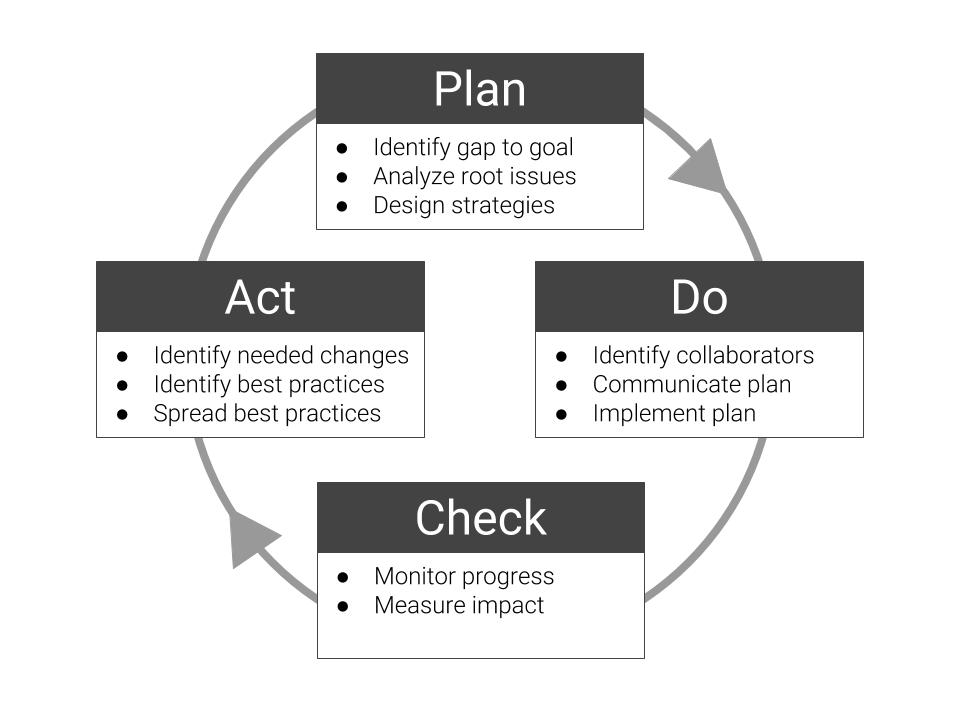
\includegraphics[width=24in]{_bookdown_files/img/pdca} \end{figure}

The table below illustrates the relationship between the PDCA process and a fuller definition of the PCP process:

\begin{table}

\caption{\label{tab:unnamed-chunk-3}Alignment of PDCA and PCP}
\centering
\begin{tabular}[t]{l|l|l|l|l}
\hline
Factor & Plan & Do & Check & Act\\
\hline
*Questions* & What is your life like? & What are you working on? & Is life better? & What next?\\
\hline
 & What do you want to pursue? & How are supports provided? &  & How to improve approach?\\
\hline
 & What supports do you need? & Where do you live/work? &  & \\
\hline
*Activities* & Identify QoL & Work on plan & Check QoL & Revise plan\\
\hline
 & Assess needs & Coordinate services & Reassess needs & (Repeat cycle)\\
\hline
 & Develop plan &  &  & \\
\hline
*Quality area* & Structure & Process & Outcome & (Re)structure\\
\hline
\end{tabular}
\end{table}

While there are various other rubrics related to learning and improvement, PDCA has been selected here because of its use of `planning' language, its simplicity, and its familiarity among behavioral healthcare providers and funders. Note that, while the questions above can be tied to various data-points, it is more important that they should be conversational: founded upon an ongoing process of personal striving for improvement.

\hypertarget{bok}{%
\chapter{A Common Body of Knowledge}\label{bok}}

A foundational effort has been working to develop a shared repository of key terms and concepts, their definitions, and how they are related to one another. This common language has the following key features:

\begin{itemize}
\tightlist
\item
  Relates all terminology back to the person, who is at the center
\item
  Includes concepts related to the PCP process, as broadly defined above, as well as common attributes for understanding the person\footnote{Note that the body of knowledge is not intended to classify services and supports.}
\item
  Promotes consistency in implementation and training, and the scalability of future development
\item
  Allows for change; the language can be extended as new concepts are identified.\footnote{This approach also requires that ideas claiming to be new must differentiate themselves from existing terms and concepts.}
\item
  Reduces confusion across various policies with inconsistent terminology and scope
\end{itemize}

\hypertarget{what-is-a-body-of-knowledge}{%
\section{What is a Body of Knowledge?}\label{what-is-a-body-of-knowledge}}

\begin{quote}
``If you wish to converse\ldots{} define your terms.''

--- Voltaire
\end{quote}

While person-centered thinking and planning is important enough to be ensconced in policy and regulation, it is also important enough that is should never become rote, and continue to be a part of a living dialogue. Both dialogue and consistent implementation require a shared language.\footnote{According to Will Durant, this requirement is ``the heart and soul of {[}logic{]}, that every important term\ldots{} be subjected to strictest scrutiny and definition. It is difficult, and ruthlessly tests the mind; but once done it is half of any task.'' (cf.~\emph{The Story of Philosophy}, New York, Garden City, 1926, p.~67)} Our purpose here is to identify and define concepts related to person-centered planning by making use of the existing legacy of policy and guidance related to person-centered planning. This will be done in a way which connects core concepts to both state and federal regulations. The collection of core concepts will serve as the foundational outline for a body of knowledge; an evolving outline of understanding about person-centered thinking, planning, implementation and monitoring.\footnote{Please note that the current work aims at an initial proof-of-concept, and not as a process ready for automation or scaling.}

\hypertarget{potential-uses}{%
\section{Potential Uses}\label{potential-uses}}

The potential uses of this body of knowledge include the following:

\begin{itemize}
\tightlist
\item
  \emph{Policy Search}: searching of existing policies in electronic format to allow for identification of requirements related to each key concept
\item
  \emph{Impact of Policy Changes}: identification of relevant new federal policy requirements to allow for clear understanding of which current policies are related and complicated by the new federal policy
\item
  \emph{Basis of Curriculum}: serving as the foundation of a standard curriculum to train people receiving services, their families, direct-care team members, supports coordinators, case managers, clinicians, and others about the PCP process.
\item
  \emph{Monitoring Quality}: allowing for system-level monitoring of the quality of PCP practice, through measurements and/or the use of a best practice review model.\footnote{This could be developed similar to the MI-FAST model, which has been used to review the fidelity to evidence-based practices.}
\item
  \emph{Promising Practices}: use of key terms for ongoing literature review and meta-analysis of PCP-related practices in the research literature, to build a base of best practices and evidence for effectiveness
\end{itemize}

\hypertarget{defining-core-concepts}{%
\section{Defining Core Concepts}\label{defining-core-concepts}}

\hypertarget{identify-core-concepts}{%
\subsection{Identify Core Concepts}\label{identify-core-concepts}}

In order to begin compiling relevant policies and guidance related to person-centered planning, we needed to select and define an initial set of core concepts related to person-centered planning. The `source of truth' for these concepts was state-level policy in Michigan, since this is the level at which shared dialogue and consistent implementation are sought.

The following method was used to develop this initial set of core concepts:\footnote{For more complete documentation, see the appendix regarding \protect\hyperlink{methods}{Detailed Methods}.}

\begin{itemize}
\tightlist
\item
  \textbf{Manual review and annotation} of a set of core documents which define person-centered planning in the Michigan Public Behavioral Health System. These include (a) the \href{https://www.michigan.gov/documents/mdhhs/Person_Centered_Planning_Policy_rev._6-17-17_597318_7.pdf}{Person-Centered Planning Policy}, (b) the \href{https://www.michigan.gov/documents/SelfDeterminationPolicy_70262_7.pdf}{Self-Determination Policy and Practice Guideline}, and (c) the Michigan Mental Health Code section \href{http://legislature.mi.gov/doc.aspx?mcl-330-1712}{330.1712 Individualized written plan of services}.
\item
  \textbf{Identifying synonyms} for core concepts. For instance, the term \emph{person} was mapped to the similar terms \emph{person, personal, patient, individual, client, consumer, recipient, beneficiary}. This is being done for all core concepts in order to flag their occurrence across multiple policies.
\item
  \textbf{Comprehensive annotation} of electronic text data for the policies referenced above, to assure that the most commonly used terms and phrases were included as core concepts.
\end{itemize}

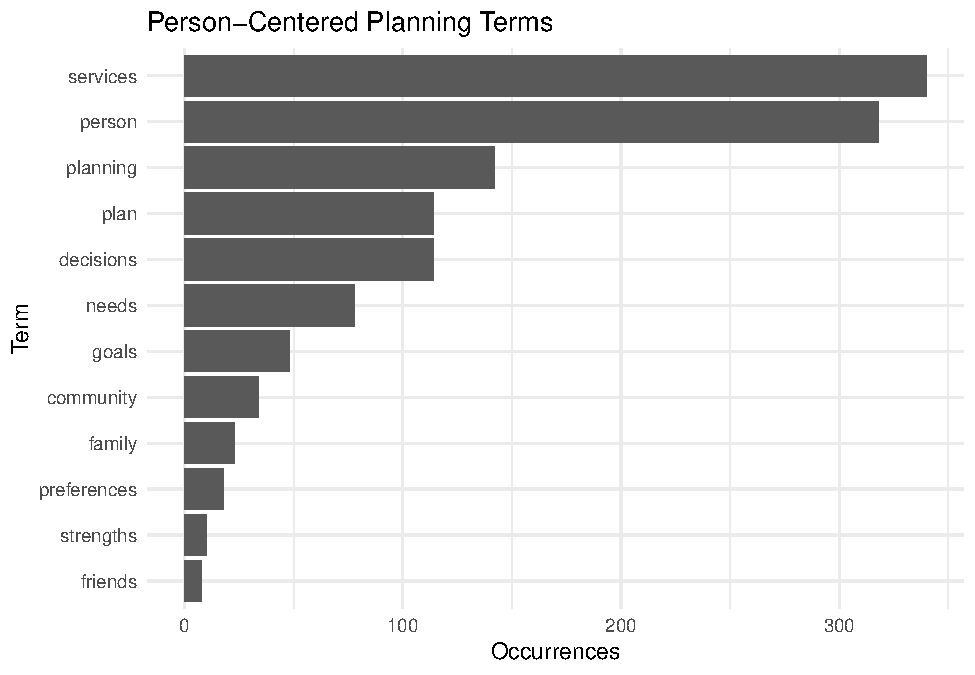
\includegraphics{person_centered_files/figure-latex/plot_concept-1.pdf}

\textbf{Purposeful Word Choice.} When we map multiple terms together as a concept, we inevitably need to select a single `master' term to refer to synonyms and identify their locations across documents with varying authors, terminology, points of view and contexts for implementation. The selection of terms is purposefully opinionated, and attempts to reflect the spirit of person-centered planning defined in the state's policy. For instance, the term `person' is prefered to various other terms, since these terms tend to view the person from only one vantage point: a participant in an economic exchange, a person requiring help from others, an individual person separated of ties to others. So, while we need to find instances where these words occur in policy, the body of knowledge also intends to approach those policies with a consistent point of view, informed by a consistent set of principles.

\textbf{Characteristics of a Person.} To put the person at the center of the language used, and to do so in way which promotes simplicity, we needed to bring some of the concepts from policy underneath a broader set of terms. With the \textbf{person} as the starting point, we define each person as having the following features:

\begin{itemize}
\tightlist
\item
  \textbf{definition}: a set of characteristics specific to that person, defined by the person and those who know them well.
\item
  \textbf{connections}: the people, places and things which make up the context of a person's life
\item
  \textbf{direction}: what a person intends for their life to become, by imagining a future and making choices to move toward it
\end{itemize}

Note that these are features of being human for all of us.

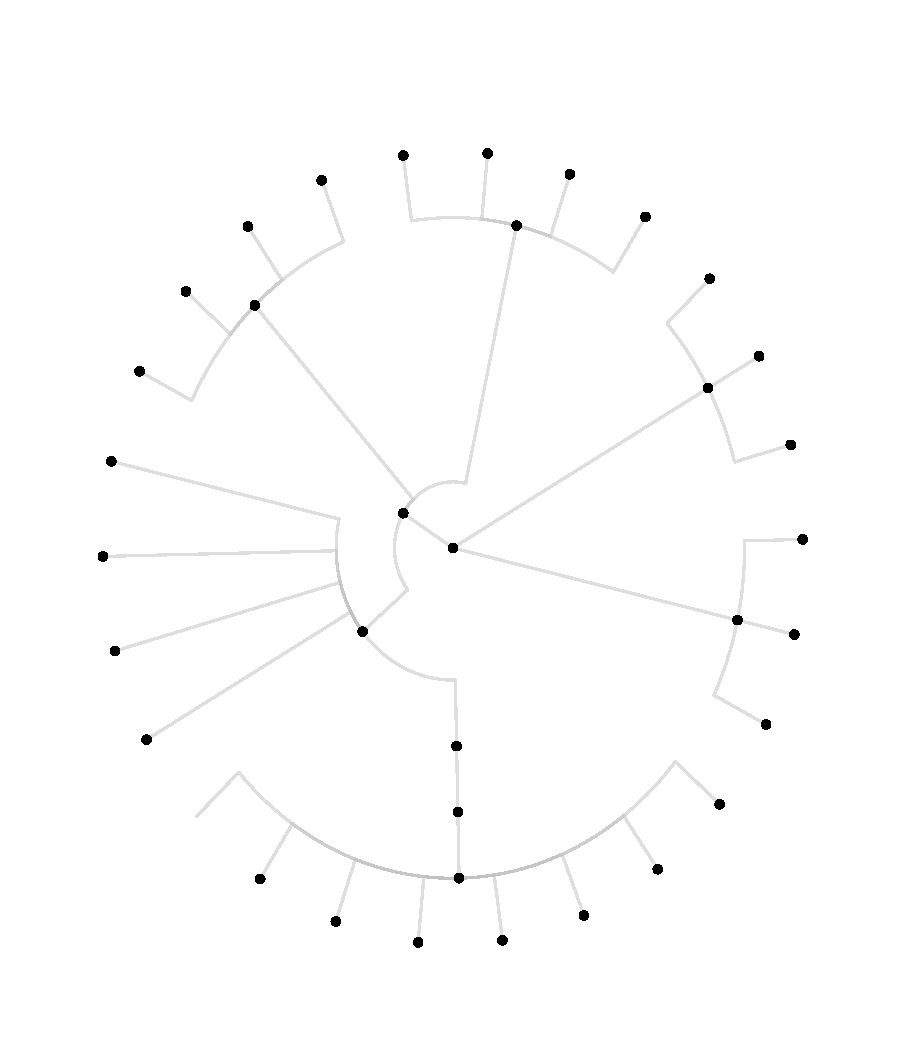
\includegraphics{person_centered_files/figure-latex/unnamed-chunk-5-1.pdf}

\hypertarget{define}{%
\section{Define Core Concepts}\label{define}}

Defining core concepts and terms, using policy where possible.

\hypertarget{policy}{%
\chapter{Comprehensive Mapping to Policy}\label{policy}}

As with any important idea, person-centered planning has been discussed and debated for decades, leaving a vast body of policy, regulations, guidance, and explanations to sift through. While many of the basic ideas of person-centered planning are simple and commonsense, practitioners are also required to adhere to existing policies. With this in mind, the body of knowledge is being developed:

\begin{itemize}
\tightlist
\item
  Based on a broad scope of relevant state and federal policies identified by MDHHS-BHDDA.
\item
  Using natural-language processing techniques to identify and refine core terminology from the text of the identified policies
\item
  In a manner that allows MDHHS-BHDDA to identify whether new federal policies would align with the current implementation of PCP
\end{itemize}

\hypertarget{identify-scope-of-policy}{%
\section{Identify Scope of Policy}\label{identify-scope-of-policy}}

In collaboration with policy experts at MDHHS-BHDDA, we identified an initial scope for the inclusion of state and federal regulations in our search. While it is designed to be extendable to include new policies as they are developed, and to allow for sharing and implementation across MDHHS departments if required, this initial set of regulations was used:

\begin{table}

\caption{\label{tab:unnamed-chunk-6}Regulations included in PCP body of knowledge.}
\centering
\begin{tabular}[t]{l|l|l}
\hline
Source & Abbreviated Title & Regulation\\
\hline
MI-State & Self-D & Self-Determination Policy \& Practice ...\\
\hline
MI-State & PCP & Person-Centered Planning\\
\hline
MI-State & MHCode & Mental Health Code\\
\hline
MI-State & Mcaid-PM & Medicaid Provider Manual\\
\hline
MI-State & AFC-TA & Adult Foster Care Group Homes Technic...\\
\hline
MI-State & AFC-SC & Certification of Specialized Programs...\\
\hline
MI-State & AFC-Act & AFC Facility Licensing Act 218 of 1979\\
\hline
MI-State & AFC-12 & Licensing Rules for AFC Small Group H...\\
\hline
Federal & Parity & Medicaid and Children's Health Insura...\\
\hline
Federal & No-Wrong-Door & Agency Information Collection Activit...\\
\hline
Federal & MU-Medicaid & Medicare Program; Hospital Inpatient ...\\
\hline
Federal & MU-EHR & 2015 Edition Health Information Techn...\\
\hline
Federal & MH-BG & Mental Health Block Grants\\
\hline
Federal & MCMC-Rx & Medicare and Medicaid Programs; Polic...\\
\hline
Federal & Mcare-Adv & Agency Information Collection Activit...\\
\hline
Federal & Mcare-ACO-Waiver & Medicare Program; Medicare Shared Sav...\\
\hline
Federal & Mcare-ACO-Savings & Medicare Program; Medicare Shared Sav...\\
\hline
Federal & Mcaid-ManagedCare & Medicaid and Children's Health Insura...\\
\hline
Federal & LTC-Reform & Medicare and Medicaid Programs; Refor...\\
\hline
Federal & HCBS & Medicaid Program; State Plan Home and...\\
\hline
Federal & ELTSS & Medicaid and Children's Health Insura...\\
\hline
Federal & Discharge & Medicare Program; Hospital Inpatient ...\\
\hline
Federal & CCHBC & CCHBC Requirements\\
\hline
Federal & ACA-Market- & Patient Protection and Affordable Car...\\
\hline
Federal & ACA-Benefit & Patient Protection and Affordable Car...\\
\hline
\end{tabular}
\end{table}

This is intended to be an initial set of policies and regulations, which can be extended as necessary.\footnote{For example, using the Federal Register API to \href{https://www.federalregister.gov/documents/search?conditions\%5Bagencies\%5D\%5B\%5D=centers-for-medicare-medicaid-services\&conditions\%5Bagencies\%5D\%5B\%5D=health-and-human-services-department\&conditions\%5Bagencies\%5D\%5B\%5D=substance-abuse-and-mental-health-services-administration\&conditions\%5Bterm\%5D=person-centered\&conditions\%5Btype\%5D\%5B\%5D=RULE\#}{search for policies} containing the phrase ``person-centered'' by relevant agencies.} Additional work will be needed to assure that the most current version of amended policies is used, as this approach is refined.

\hypertarget{find-occurrence-of-concepts-in-policy}{%
\section{Find Occurrence of Concepts in Policy}\label{find-occurrence-of-concepts-in-policy}}

The core concepts are derived from \protect\hyperlink{policy}{key policy documents}, and related terms can be flagged within other policy documents.

To do this, we take the annotated version of the regulation and replace words and phrases with their corresponding concepts. We then reconstitute the original document with these replacements.

\hypertarget{research}{%
\chapter{Informed by (and Informing) Research}\label{research}}

Some activities related to person-centered planning are addressed in existing research.\footnote{For instance, \emph{goals and planning}, \emph{feedback and monitoring}, and similar activities defined by the \href{https://www.humanbehaviourchange.org/resources/behavioural-science/25/description}{Behaviour Change Intervention Ontology (BCIO)} have related research available.} In these instances, our goal would be to connect-the-dots between research and practice by making this knowledge available. In order to remain aligned with national efforts\footnote{NQF's \href{http://www.qualityforum.org/WorkArea/linkit.aspx?LinkIdentifier=id\&ItemID=91382}{Person-Centered Planning and Practice Project}, references `\emph{a research agenda to advance and promote person-centered planning in LTSS}'} in this area, initial steps would include:

\begin{itemize}
\tightlist
\item
  mapping of person-centered planning concepts to researched interventions, where these exist
\item
  use of key concepts from the body of knowledge for literature review and meta-analyses of PCP-related practices, to build a base of best practices and evidence for effectiveness
\item
  identification of gaps in existing research knowledge related to PCP
\end{itemize}

\hypertarget{curriculum}{%
\chapter{Shared Training Curriculum}\label{curriculum}}

To translate this common body of knowledge into action, various audiences need to be trained in the core elements of person-centered practice, using the foundational concepts identified and defined above. Work in developing these trainings includes:

\begin{itemize}
\tightlist
\item
  Identification of key audiences
\item
  Evaluation of potential training modalities based on key features
\item
  Developing a standard base curriculum as well as specialty topics for specific audiences
\end{itemize}

\hypertarget{measure}{%
\chapter{Person-Centered Measurement Framework}\label{measure}}

If the entire system of services and supports is intended to be person-centered, its performance should be measured within a framework that is centered on the person. Since many existing quality measures and data collection systems were not developed with this in mind, it will be important to develop a larger framework within which existing measures can be situated. This allows the system to retain the quality measurement work that has been completed, while acknowledging gaps within that framework which need to be filled.

The framework outlined here attempts to align with and fulfill the promise of current definitions of person-centered planning, as well as with existing and evolving standards in the fields of behavioral health and developmental disability services. Far from contradicting these standards, it attempts to provide a broader, person-centered context for the development of the system as a whole.

Ongoing work in this area would include:

\begin{itemize}
\tightlist
\item
  Developing a person-centered measurement framework
\item
  Conducting an inventory of available data assets at a state wide level
\item
  Classifying existing measurement and data collection efforts (e.g.~HEDIS, BH-TEDS, etc.) within the context of this framework
\end{itemize}

\hypertarget{what-do-we-mean-by-a-better-life}{%
\section{What do we mean by `a better life'?}\label{what-do-we-mean-by-a-better-life}}

People have been asking themselves what it means to live a good life for thousands of years,\footnote{The philosopher Aristotle defined the highest good of human life as happiness, or flourishing (\emph{eudaimonia}). cf.~\emph{Nicomachean Ethics}} and it is among the most crucial questions for each of us to answer. Here, we will refer to the characteristics that make up a good life as \emph{quality of life}, or QOL for short, relying primarily on contemporary research to arrive at a common and usable definition.

\hypertarget{what-makes-a-good-definition}{%
\subsection{What makes a good definition?}\label{what-makes-a-good-definition}}

If we are going to try to define quality of life, it is important that our definition gets a few things right:\footnote{These considerations are drawn from \href{https://www.ncbi.nlm.nih.gov/pubmed/16162114}{Cummins, R. (2005). Moving from the quality of life concept to a theory. JIDR, 49(10), 699-706}.}

\begin{enumerate}
\def\labelenumi{\arabic{enumi}.}
\tightlist
\item
  \emph{Multiple dimensions}. A good life can only be described using multiple dimensions. These are influenced by personal factors, environmental factors, and the interaction between those factors.
\item
  \emph{Broad enough for everyone}. We should each want to apply the definition to our own lives. The basic characteristics of a good life are the same for all people, regardless of culture, gender, disability, etc.
\item
  \emph{Both subjective and objective}. People have different priorities. While a definition can point to objective facts related to QoL, it must include the point-of-view of the person who is living their life from day to day. Each dimension of a QoL model may have both objectively and subjectively defined indicators.
\end{enumerate}

Taken together, the criteria listed above seek to balance the abstract with the specific to arrive at a definition which is well-rounded and understandable.

\hypertarget{what-makes-a-better-life}{%
\subsection{What makes a better life?}\label{what-makes-a-better-life}}

Keeping our key requirements in mind, we can draw from the broad reservoir of studies on QoL to find frameworks which are multi-dimensional\footnote{See systematic review of HRQoL recommending addition of individual and environmental characteristics: \href{https://www.ncbi.nlm.nih.gov/pmc/articles/PMC3548743/}{Bakas, T., et al.~(2012)}.}, cross-culturally relevant,\footnote{See \href{https://www.researchgate.net/profile/Mian_Wang4/publication/7801771_Cross-Cultural_Study_of_Quality_of_Life_Indicators/links/0deec52df448eac34d000000/Cross-Cultural-Study-of-Quality-of-Life-Indicators.pdf}{Schalock, R., et al.~(2005).}.} and which provide both subjective and objective indicators.

Below is a potential model listing essential dimensions of QoL:

\begin{table}

\caption{\label{tab:unnamed-chunk-8}QoL Dimensions}
\centering
\begin{tabular}[t]{l|l|l}
\hline
Area & Dimension & Example Indicators\\
\hline
Independence & Personal development & Education status, personal skills, ADLs, IADLs\\
\hline
 & Self-determination & Choices, autonomy, personal control, goals\\
\hline
Social participation & Interpersonal relations & Social networks, activities, relationships\\
\hline
 & Social inclusion & Community integration, participation, roles\\
\hline
 & Rights & Human (respect/dignity, equality), Legal\\
\hline
Well-being & Emotional well-being & Safety, positive experiences, self-concept, stress\\
\hline
 & Physical well-being & Health, nutrition, recreation/physical exertion\\
\hline
 & Material well-being & Financial status, employment, housing, possessions\\
\hline
\end{tabular}
\end{table}

Please note that the framework listed above is one of many potential models, each of which contains many of the same basic dimensions, and many were developed with populations having specific conditions. Some other broad-based models for review include:

\begin{itemize}
\tightlist
\item
  The \href{https://apps.who.int/iris/bitstream/handle/10665/77932/WHO_HIS_HSI_Rev.2012.03_eng.pdf?sequence=1\&isAllowed=y}{World Health Organization Quality of Life (WHOQOL)} domains.
\item
  The \href{https://ec.europa.eu/eurostat/statistics-explained/index.php?title=Quality_of_life_indicators}{Eurostat QoL indicators} show an example of QoL domains applied for entire countries alongside financial indicators such as gross domestic product (GDP).
\item
  Healthy People 2020 has selected a subset of measures for monitoring health-related QoL and well-being in the United States. See their \href{https://www.healthypeople.gov/sites/default/files/HRQoLWBFullReport.pdf}{Foundation Health Measure Report: Health-Related QoL and Well-Being}.
\end{itemize}

\hypertarget{benefits-of-a-qol-perspective}{%
\section{Benefits of a QoL Perspective}\label{benefits-of-a-qol-perspective}}

\hypertarget{what-other-frameworks-exist}{%
\subsection{What other frameworks exist?}\label{what-other-frameworks-exist}}

One might well ask: \emph{Is quality of life the only potential framework that we could use to measure improvement?} The answer is \emph{No}, so it is worth discussing other options and briefly reviewing the attributes of each. Other options include:

\begin{itemize}
\tightlist
\item
  \emph{Symptom reduction}: Measurement of reduction in symptoms related to specific diagnosable conditions. Symptom scales such as the \href{https://www.phqscreeners.com/sites/g/files/g10049256/f/201412/PHQ-9_English.pdf}{PHQ-9}, \href{}{GAD-7} and other tools have commonly been used to measure the impact of treatments on specific conditions, but they are more challenging to use for people with multiple co-occuring conditions (MCC).
\item
  \emph{Improving functional status}: Most currently used assessment tools address functional status, measuring the impact of various conditions on broader life areas in terms of their impact on functional ability. These are broader than symptom scales, and can detect the impact of various symptoms on a particular functional domain.
\item
  \emph{Health-related quality of life (HRQoL)}: HRQoL addresses a subset of QoL domains which are related to perceived physical and mental health. These models typically exclude non-medical areas such as education or rights, focusing on physical domains like `mobility'.
\end{itemize}

\hypertarget{why-is-a-quality-of-life-framework-better-than-others}{%
\subsection{Why is a quality of life framework better than others?}\label{why-is-a-quality-of-life-framework-better-than-others}}

A QoL approach has the following benefits over the approaches mentioned above:

\textbf{Strengths-based}: A QoL approach asks people what they want their lives to be and encourages them to work toward that vision. Rather than focusing on needs or deficits, it aspires to use a person's strengths to improve his or her life.\footnote{See the MDHHS PCP Policy value that ``The PCP approach identifies the person's strengths, goals, choices\ldots{} and desired outcomes.'' (p.~4)}

\textbf{Inclusive}: Instruments and measures from each of the other areas can be used as a part of the QoL framework, since it is broad enough to include each of these areas, and they each contribute to it. A QoL approach does not neglect the value of functional gains or symptom reduction, but values these as contributors to overall quality of life. For instance, if a person experiences an alleviation of their depressive symptoms using the PHQ-9, this would be seen as contributing toward the individual's QoL in the area of `Emotional Well-being'.

\textbf{Contextual}: An approach which focuses on only a portion of an individual's life, such as mobility or anxiety symptoms, is likely to miss out on the bigger picture. It may also inadvertently create siloes among the individuals supporting the person. For instance, more recent evaluations have criticized the HRQoL approach as failing to ``sufficient emphasis on mental and social domains\ldots{}that are essential to people.''\footnote{Read \href{https://www.ncbi.nlm.nih.gov/pmc/articles/PMC4031380/}{Pietersma, S., et al.~(2013)} regarding domains of quality of life.} The broader focus on QoL which is proposed here is aligned with our evolving understanding of several areas, each of which stresses the critical relationship between each of us and our communities and surroundings:

\begin{itemize}
\tightlist
\item
  \emph{Social Determinants of Health} (SDoH): A vast and growing body of \href{https://www.cdc.gov/socialdeterminants/research/index.htm}{research} indicates that the places and conditions in which we live are intrinsically tied to the quality of our lives and the likelihood of achieving positive outcomes from the supports and services we receive.
\item
  \emph{Trauma-Informed Care}: More and more models for service provision, informed by research and by the lived experience of trauma survivors, are founded on the recognition that adverse events in our relationships and in our lived environment can have a profound and lifelong impact on our lives.\footnote{For a recent review of these models, see: \href{https://www.ncbi.nlm.nih.gov/pubmed/30079827}{Purtle, J. (2018). Trauma, Violence, \& Abuse}.}
\item
  \emph{Supports Paradigm}: A model, prevalent in the IDD supports system, that views a person's functioning as the match between their individual capacity and the environment in which they are expected to live and work.\footnote{See \href{https://www.ncbi.nlm.nih.gov/pubmed/19368481}{Thompson, et al.~(2009)} on conceptualizing support needs.} In this model, supports are viewed as a way to supplement the persons strengths and to help match those to the person's environment.
\end{itemize}

\hypertarget{alignment-with-existing-requirements}{%
\section{Alignment with Existing Requirements}\label{alignment-with-existing-requirements}}

\hypertarget{alignment-with-federal-medicaid-requirements}{%
\subsection{Alignment with Federal Medicaid Requirements}\label{alignment-with-federal-medicaid-requirements}}

\hypertarget{alignment-with-provider-requirements}{%
\subsection{Alignment with Provider Requirements}\label{alignment-with-provider-requirements}}

\emph{Feasible for Implementation}: Multiple pragmatic trials have demonstrated that the use of symptom scales are both feasible to implement on a large scale\footnote{See the large scale implementations cited in \href{https://ps.psychiatryonline.org/doi/full/10.1176/appi.ps.201500439\#T1}{Fortney, J. C., et al.~(2016). A tipping point for measurement-based care. Psychiatric Services, 68(2), 179-188.}.} and acceptable to people receiving services.\footnote{\href{https://www.bmj.com/content/338/bmj.b663.long}{Dowrick, C., et al.~(2009)} report that the use of instruments increase confidence in providers' accuracy and management.}

\emph{Provider Accreditation}: New standards for Joint Commission accreditation (effective 2018)\footnote{See Joint Commission \href{https://www.jointcommission.org/assets/1/6/Approved_BHC_outcome_meas_2018.pdf}{\emph{Standard CTS.03.01.09}, sections \emph{EP1-3}}.} require that an organization (a) ``uses a standardized tool or instrument to monitor individuals progress in achieving\ldots{} goals'', (b) ``gathers and analyzes data generated through standardized monitoring, and results used to inform goals and objectives of individual's plan'', and (c) ``evaluates outcomes of\ldots{} services\ldots{} by aggregating and analyzing data collected through the standardized monitoring effort.''

\emph{Diagnostic Practice}: The most recent diagnostic manual (DSM-5) includes \href{https://www.psychiatry.org/psychiatrists/practice/dsm/educational-resources/assessment-measures}{assessment measures} which were ``developed to be administered at the initial patient interview and to monitor treatment progress.''

\hypertarget{framework-for-measurement}{%
\section{Framework for Measurement}\label{framework-for-measurement}}

\hypertarget{scope}{%
\subsection{Scope}\label{scope}}

\begin{figure}
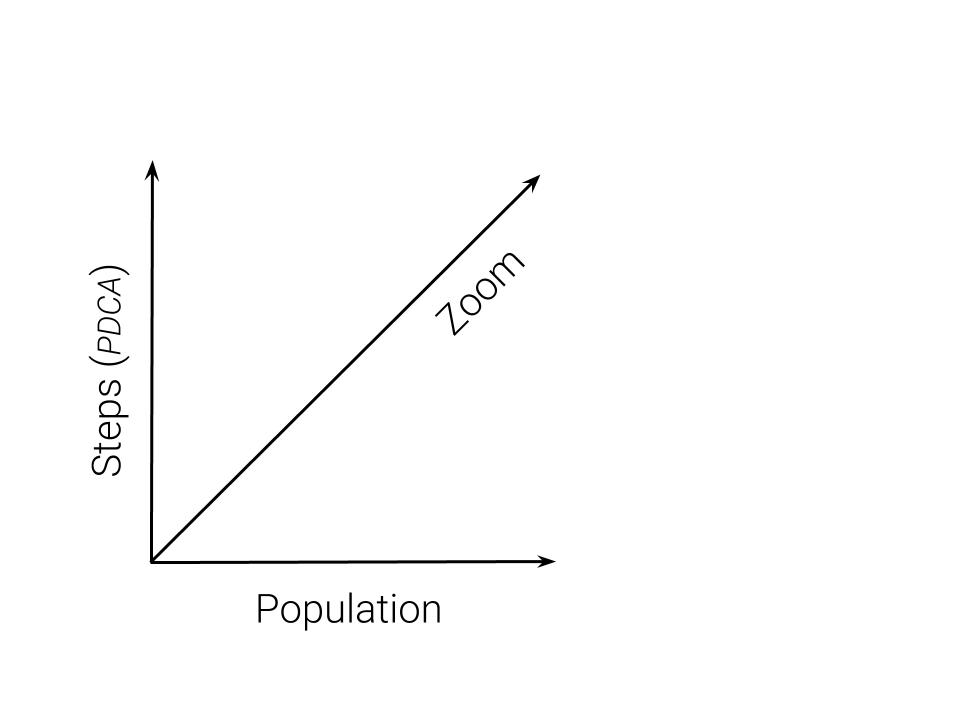
\includegraphics[width=24in]{_bookdown_files/img/QoL Framework Scope} \caption{Scope of framework}\label{fig:unnamed-chunk-9}
\end{figure}

A conceptual framework as comprehensive as the one we are proposing runs the risk of becoming overwhelmingly complex and unwieldy to implement. So, before diving into any details, we want to begin by sketching out a simple way to think about the scope of the framework required to systematically measure person-centered planning and its impact of quality of life. Having a definition of scope can help us answer questions such as:

\begin{itemize}
\tightlist
\item
  What types of data are included, and what types of measures?\\
\item
  How will we know when the framework is fully implemented?\\
\item
  Does this fit with other work that we are doing?
\end{itemize}

We can define the scope of the framework using three-dimensions (\emph{\protect\hyperlink{zoom}{depth}, \protect\hyperlink{pop}{breadth}, and \protect\hyperlink{steps}{height}}) as defined below:

\textbf{Depth} (a.k.a. \emph{Zoom}): Does the framework allow for understanding at various levels of `resolution', from the most immediate (i.e.~\emph{the individual person}) to the aggregate (i.e.~\emph{the population}) and other levels inbetween (e.g.~\emph{the organization, team, etc.})?

\textbf{Breadth} (a.k.a. \emph{Population}): Can the framework apply to all people who are planning to improve their lives with the help of services and supports?\footnote{I.e., to all `populations' around which systems have been developed (\emph{SMI, SED, IDD, SUD, etc.}). Since different data exists for each group, evaluating alignment is key.}

\textbf{Height} (a.k.a. \emph{Steps}): Does the framework allow for understanding of each of the steps in the \protect\hyperlink{pcpdca}{person-centered PDCA process} discussed above?

\begin{figure}
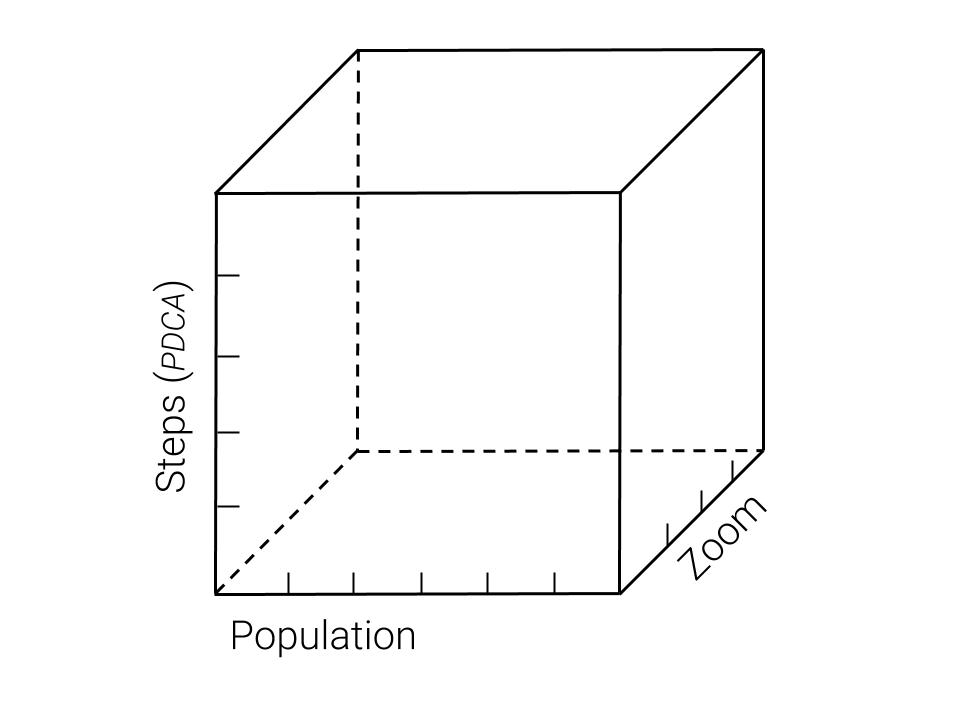
\includegraphics[width=24in]{_bookdown_files/img/QoL Framework Cube} \caption{If it was a cube...}\label{fig:unnamed-chunk-10}
\end{figure}

If we think about the framework as a cube made of these three dimensions, then developing the measurement framework can begin by making certain that data is collected:

\begin{itemize}
\tightlist
\item
  at each step of the person-centered PDCA process (\emph{height})
\item
  for people across all populations (\emph{breadth})
\item
  which can be aggregated at various levels of the system (\emph{depth})
\end{itemize}

So, speaking \emph{very} broadly, if our cube has data elements/measures at each intersection of the three dimensions, then it allows for at least a basic understanding of people's needs, planning, and services as these contribute to improved lives. In reality, there will always be additional data that can be collected and novel ways of combining that data, just as there continue to be additional books and songs written describing the human experience.

The next sections define each of the dimensions listed above, and how they relate to one another, in greater detail. Based on these details, it will be possible to begin a practical gap analysis to assess how closely the system's current data assets match the scope of the framework. Please note that this paper does not develop or identify specific measures, except as illustrations of how individual data elements or metrics \emph{might} fit into the overall framework.

\hypertarget{steps}{%
\subsection{Steps}\label{steps}}

\hypertarget{plan}{%
\subsubsection{Plan}\label{plan}}

\textbf{Understand Quality of Life.}

\textbf{Understand Needs Related to QoL.} The table below identifies example variables from required assessments which relate to the QoL domains outlined above.\footnote{Assessments included are the \href{http://aaidd.org/sis}{\emph{Supports Intensity Scale (SIS)}}, the \href{http://www2.fasoutcomes.com/Content.aspx?ContentID=12}{\emph{Child and Adolescent Functional Assessment Scale (CAFAS)}}, the \href{https://cchealth.org/mentalhealth/pdf/LOCUS.pdf}{\emph{Level of Care Utilization System (LOCUS)}}, and the \href{http://gaincc.org/}{\emph{Global Appraisal of Individual Needs (GAIN)}}} While this is not an exhaustive mapping, it shows how the assessment of personal needs (\emph{from the ``Plan'' step of PDCA}) relate to quality of life domains across multiple populations.

\begin{table}

\caption{\label{tab:unnamed-chunk-11}Sample: Need Assessment and Related QoL Dimensions}
\centering
\begin{tabular}[t]{l|l|l|l|l}
\hline
Dimension & SIS Subscale & CAFAS Item & LOCUS Item & GAIN Item\\
\hline
Personal development & Health \& Safety & School/Work &  & \\
\hline
 & Protection/Advocacy & Thinking &  & \\
\hline
 & Behavioral Support &  &  & \\
\hline
Self-determination & Protection/Advocacy &  & Engagement & \\
\hline
Interpersonal relations & Social Activities & Home &  & \\
\hline
Social inclusion & Community Living & Community &  & Living Situation\\
\hline
 & Social Activities &  &  & Environment\\
\hline
Rights & Protection/Advocacy &  &  & Legal\\
\hline
 & Health \& Safety &  &  & \\
\hline
Emotional well-being & Behavioral Support & Moods/Emotions & Risk of Harm & Emotional health\\
\hline
 & Health \& Safety & Behavior &  & \\
\hline
Physical well-being & Medical Support & Self-Harm & Co-Morbidity & Physical health\\
\hline
 & Health \& Safety &  & Risk of Harm & Disease prevention\\
\hline
Material well-being & Employment & Material Needs &  & Vocational\\
\hline
\end{tabular}
\end{table}

As mentioned above, the table above is intended to illustrate how assessments of need can be tied to QoL domains, but is not comprehensive.\footnote{For the SIS instrument, this table relied on the mapping described in \href{https://biblio.ugent.be/publication/1169626/file/6748818.pdf}{Van Loon, J., et al.~(2010). \emph{Assessing individual support needs to enhance personal outcomes}. Exceptionality, 18(4), 193-202}.} The actual mapping will need to be done at the level of specific questions, as opposed to subscales which are not as likely to fit neatly within a single QoL domain. Note that instruments which contain a larger number of items (such as the SIS) are likely to have greater coverage of QoL domains than instruments with a smaller number of items (such as the LOCUS).

\hypertarget{do}{%
\subsubsection{Do}\label{do}}

\hypertarget{check}{%
\subsubsection{Check}\label{check}}

When are measures taken?

What types of measures relate to what parts of the PCP process?

\hypertarget{act}{%
\subsubsection{Act}\label{act}}

\hypertarget{pcp-based-episodes}{%
\subsubsection{PCP-based Episodes}\label{pcp-based-episodes}}

Improvement takes time, both in our personal lives and in our collective work as organizations and systems. Various frameworks have been developed to help evaluate improvement over time, many of which rely on the concept of ``episodes'': periods of time which characterized by specific events or attributes. For instance\ldots{}

\begin{itemize}
\tightlist
\item
  an admission to treatment is used to define an episode in the \emph{Substance Abuse and Mental Health Services Administration} (SAMHSA) \href{https://www.samhsa.gov/data/data-we-collect/teds-treatment-episode-data-set}{\emph{Treatment Episode Data Set} (TEDS)}
\item
  the course of a particular illness is used to define an episode in the \emph{National Quality Forum}'s \href{https://www.qualityforum.org/Publications/2010/01/Measurement_Framework__Evaluating_Efficiency_Across_Patient-Focused_Episodes_of_Care.aspx}{Patient-Focused Episodes of Care}
\end{itemize}

Neither of the approaches above is optimal for understanding the effectiveness of the implementation of a person-centered plan. The admission-based approach will create longer episodes for long-term services and supports which do not correspond to revisions of the person-centerd plan and the effect of those revisions on quality of life. The illness-based approach will be overly reductive for people with multiple, concurrent conditions, lifelong conditions, or whose social and environmental conditions have a strong adverse impact on their quality of life.

If the person-centered planning (and doing, checking, acting) process is to be the primary catalyst for improvement of life using Medicaid supports and services, then that process should be used to define episodes for improvement. The `episode' of a PCP cycle would correspond to the period of time between the plan and its next subsequent revision. If person-centered planning is expected to be creative, collaborative, and dynamic, then different `visions and revisions' of the plan will be longer or shorter. For instance, if a person develops a plan but soon realizes that it is not helping them to achieve the life goals they intended to, then the plan would be revised and the PCP episode would relatively short.

\hypertarget{zoom}{%
\subsection{Zoom}\label{zoom}}

\hypertarget{pop}{%
\subsection{Population}\label{pop}}

  \bibliography{book.bib,packages.bib}

\end{document}
